% ----------
% A LaTeX template for course project reports
% 
% This template is modified from "Tech Report ala MIT AI Lab (1981)"
% 
% ----------
\documentclass[12pt, letterpaper, oneside]{article}

% this makes every even page have an indent along the entire page
% \documentclass[12pt, letterpaper, twoside]{article}


\usepackage{geometry}
\usepackage[utf8]{inputenc}
\usepackage[english]{babel}
\usepackage[runin]{abstract}
\usepackage{titling}
\usepackage{booktabs}
\usepackage{fancyhdr}
\usepackage{helvet}
\usepackage{csquotes}
\usepackage{graphicx}
\usepackage{blindtext}
\usepackage{parskip}
\usepackage{etoolbox}
\usepackage{hyperref}

% images folder
\graphicspath{ {./report-images/} }

% preamble.tex

\geometry{letterpaper, top=2.2in, headheight=1.7in}
\date{}

\makeatletter

\def\fulltitle#1{\def\@fulltitle{#1}}
\def\runningtitle#1{\def\@runningtitle{#1}}
\def\runningauthor#1{\def\@runningauthor{#1}}
\def\affiliation#1{\def\@affiliation{#1}}
\def\department#1{\def\@department{#1}}
\def\memoid#1{\def\@memoid{#1}}
\def\theyear#1{\def\@theyear{#1}}
\def\mydate#1{\def\@mydate{#1}}

\runningtitle{How to write an effective report} % Short title
\author{Your name \and John Doe \and Jane Doe} % Full list of authors
\runningauthor{Your name et al.} % Short list of authors
\affiliation{Your University} % Affiliation e.g. University or Company
\department{Your Department} % Department or Office
\memoid{AI Memo 777} % ID of the tech report
\theyear{2018} % year of the tech report
\mydate{August 08, 2018} %the date

\def\displaymydate{\@mydate}
\def\displaytheyear{\@theyear}
\def\displaymemoid{\@memoid}
\def\displaydepartment{\@department}
\def\displayaffiliation{\@affiliation}
\def\displayrunningauthor{\@runningauthor}
\def\displayrunningtitle{\@runningtitle}

\makeatother

\makeatletter
\patchcmd{\@zfancyhead}{\fancy@reset}{\f@nch@reset}{}{}
\patchcmd{\@set@em@up}{\f@ncyolh}{\f@nch@olh}{}{}
\patchcmd{\@set@em@up}{\f@ncyolh}{\f@nch@olh}{}{}
\patchcmd{\@set@em@up}{\f@ncyorh}{\f@nch@orh}{}{}
\makeatother

% ----------
% fancyhdr setup
% ----------

\pagestyle{fancy}
\renewcommand{\headrulewidth}{0pt}

\fancypagestyle{firstpage}
{
    \fancyhf{}
    \fancyhead{%
        \begin{center}
            \textsc{\displayaffiliation}\\
            \textsc{\displaydepartment}
        \end{center}
        \vspace*{0.5in}
        \displaymemoid
        \hfill
        \displaymydate
    }
    \fancyfoot[L]{\footnotesize \textbf{\textsc{\displayaffiliation} -- \displaytheyear}}
}
\fancyhead[EL]{\small \displayrunningauthor}
\fancyhead[ER]{\small Page \thepage}
\fancyhead[OL]{\small Page \thepage}
\fancyhead[OR]{\small \displayrunningtitle}

\chead{}
\lfoot{}
\cfoot{}
\rfoot{}

% ----------

\providecommand{\keywords}[1]{\noindent \textbf{Keywords:} #1} % keywords definition

\renewcommand{\familydefault}{\sfdefault} % sans-serif font
\setlength{\parskip}{1em} % 1em skip between paragraphs
\abslabeldelim{:} % use colon after the run-in 'Abstract' word
\setlength{\parindent}{0pt} % no indentantion for first page 
\setlength{\abstitleskip}{-\absparindent} % this is because the abstract package sets \absparindent to \parindent

\pretitle{\Large \begin{center}}
\posttitle{\\[2ex] \Large \textbf{by}\end{center}}

% ----------
% Variables
% ----------

\title{\textbf{Computer Vision Course Project:\\ParkVision: A Real-Time Parking Management}} % Full title of your tech report
\runningtitle{ParkVision} % Short title
\author{Aaron James \and Jacob Rempel} % Full list of authors
\runningauthor{Aaron James \& Jacob Rempel} % Short list of authors
\affiliation{Ontario Tech University} % Affiliation e.g. University or Company
\department{Faculty of Science, Computer Science} % Department or Office
\memoid{Project Group: 19} % Project group ID that were shared with the class earlier.
\theyear{2025} % year of the tech report
\mydate{April 6, 2025} %the date


% ----------
% actual document
% ----------
\begin{document}
\maketitle

\begin{abstract}
    \noindent
    
    Efficient parking management is a growing challenge in many urban environments, leading to issues such as wasted time, driver frustration, and increased fuel consumption. By design, ParkVision offers a computer vision-based solution that rapidly detects vacant parking spots from an aerial perspective. Using OpenCV-based image processing, combined with a YOLO deep learning model, trained on two Kaggle datasets containing approximately 32 000 images. Designed for parking lots with standardized, well-defined markings, ParkVision determines space occupancy within a short to medium range. With a low-cost setup, such as a single camera and a Raspberry Pi, ParkVision enables the monitoring of hundreds of spaces simultaneously. Ultimately, ParkVision aims to enhance parking efficiency, reduce congestion, and provide scalable, real-time guidance for drivers in environments such as airports and urban lots.
    
\end{abstract}

\vspace{2.5cm}

% Uncomment the following to add thanks.
% {\footnotesize
%     \noindent
%     Special thanks to \textbf{Person 1} and \textbf{Affiliation A} for financial support for this project.
% }

\thispagestyle{firstpage}

\pagebreak

% ----------
% End of first page
% ----------

\newgeometry{} % Redefine geometries (normal margins)

\section{Introduction}
\label{sec:intro}

Urbanization and population growth have led to a significant increase in the number of vehicles travelling, increasing the demand for efficient parking solutions in many different environments. Drivers often waste valuable time searching for available parking spots, contributing to increased traffic congestion, fuel consumption, and environmental pollution. Traditional methods of parking lot monitoring include physical on-foot monitoring, remote gate control with assistance from a surveillance system, or most prominently, none at all. The methods involving any active monitoring can be expensive, labour intensive and difficult to scale.

Recent advancements in computer vision and deep learning offer a favourable alternative. Leveraging object detection models, and real time image processing, automation of vacancy monitoring in parking lots is achievable with visual data alone. This not only reduces infrastructure and labour costs, but enables an easy, scalable, and adaptable parking management solution.

ParkVision is a computer vision-based solution designed to detect vacant and occupied parking spots from an aerial perspective using real time image processing and deep learning. Our project uses a YOLO-based object detection model in combination with OpenCV to analyse parking lot footage to determine the vacancy status in a parking lot. ParkVision focuses specifically on parking lots with clearly defined parking lines and standardized layouts, making it easily suitable for deployment in most structured urban and commercial environments.

The overall objective of this project is to provide real-time insights into parking lot occupancy, improve traffic flow, and enhance overall efficiency of urban parking systems.

\section{Methodology}
\label{sec:methodology}
The ParkVision system is designed to detect vacant and occupied parking spots from aerial imagery using computer vision and deep learning. The data pipeline that this system uses is data preparation, model training, and real-time inference. All of these core components will be detailed throughout the following subsections.


\subsection{Dataset Preparation}

We worked with three different public datasets from Kaggle.com, which contained thousands of labelled parking lot images with corresponding annotated occupancy information. All of these datasets were first pre-processed to ensure consistency.

\begin{enumerate}
    \item All annotations were converted to YOLO format (normalized center-based bounding boxes). Bounding box coordinates were extracted from XML and JSON in some cases.

    \item The datasets were split into training, validation, and testing sets based on size. Datasets with over 10 000 images were split into 80\% training, 10\% validation, and 10\% testing. The smaller dataset (under 10 000 images) was split into 70\% training, 15\% validation, and 15\% testing. These ratios were selected based on research to optimize model performance.

    \item Bounding boxes were labelled either vacant or occupied based on the dataset annotations.
    
\end{enumerate}

  
\subsection{Model Architecture}

We used several models from the Ultralytics YOLO YOLOv11 family, including YOLOv11n, s, m, and x. YOLO (You Only Look Once) models are well suited for real time inference given the ability to process entire images in a single forward pass. This makes them an ideal choice for ParkVision, where quick and accurate results are a highlighted priority in dynamic environments.

\subsection{Occupancy Detection Logic}

Each predicted bounding box was classified as either vacant or occupied. To evaluate accuracy:

\begin{itemize}
    \item Predictions were compared with ground truth labels using Intersection Over Union (IoU).

    \item Matches above an IoU threshold of 0.5 and correct class labels are counted as True Positives.

    \item Unmatched predictions were False Positives.

    \item Unmatched ground-truth boxes were False Negatives.

\end{itemize}

\subsection{Evaluation Metrics}
The model was evaluated using the following metrics:

\begin{itemize}
    \item Precision: How many predicted occupied/vacant spots were actually correct

    \begin{itemize}
        \item High Precision = Few false positives
        \item Low Precision = Model guessing too much
    \end{itemize}

    \item Recall: How many actual occupied/vacant spots the model was able to correctly detect

    \begin{itemize}
        \item High recall = few false negatives

        \item Low recall = missing many real occupied/vacant spots

    \end{itemize}

    \item F1 Score: Harmonic mean of precision and recall

    \begin{itemize}
        \item High F1 = good balance of precision and recall

        \item Low F1 = poor performance in one or both areas

    \end{itemize}

    \item Detection Rate: Percentage of ground truth spots the model identified, as well as the models ability to locate all spaces in the image
\end{itemize}

\section{Results}
\label{sec:results}

\subsection{The PKLot Dataset}
\subsubsection{Training}

The first dataset we decided to use was \href{https://www.kaggle.com/datasets/ammarnassanalhajali/pklot-dataset}{PKLot} from Kaggle which contains approximately 700k images. The images come from three different cameras, two cameras are from the same parking lot and the third camera is from a completely different parking lot. Every image is taken at a different time of the day throughout the year, this results in a dataset that has extensive data on the different types of cars, different weather conditions, and different times of day giving a ton of brightness deviations. We converted this data set into a YOLO ready format, and commenced training on a pre-trained YOLOv11 model, with a fine tuning of 25 epochs.

\subsubsection{Overfitting and Limitations of PKLot}
Unfortunately training a YOLO model on a dataset of the same three parking lots results in a model that is \textbf{very} good at identifying parking spaces \textbf{only} in that parking lot. This is the results of the YOLOv11m model after training for 25 epochs. 

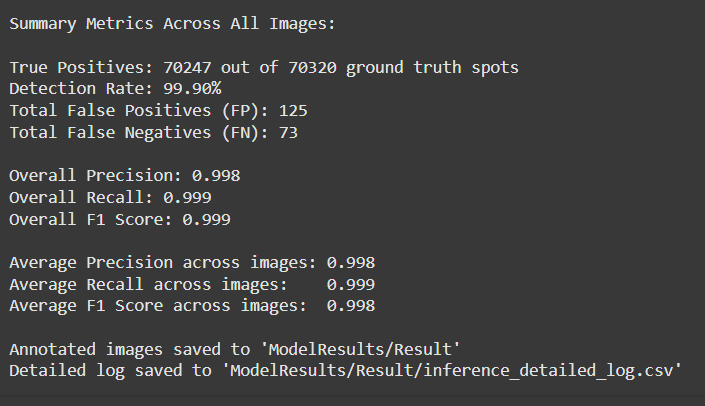
\includegraphics[scale=0.8]{pklot-25epochs-medium-results.png}

The model is clearly overfitting the data, and running it for 25 epochs only amplifies the problem. Here is the model performing inference on in domain data:

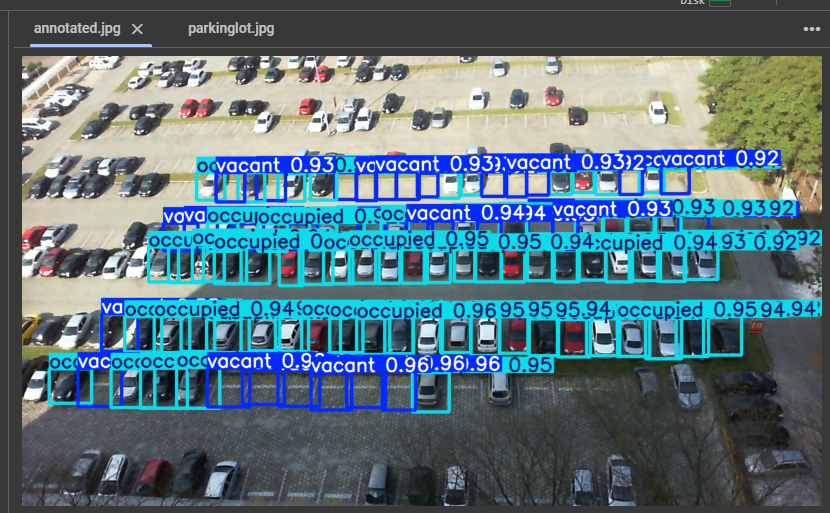
\includegraphics[scale=0.5]{report-images/pklot-25epochs-medium-inference.png}

When an out-of-domain image was selected, the model did not identify a single parking space. After reassessing the PKLot dataset, our conclusion was that the dataset lacked diversity, having nearly 700k images of essentially the same location. This model was able to perform inference very well for images of the same parking lots included inside the dataset. However, it failed to generalize to images from domains not represented in the dataset, rendering it ineffective for out-of-domain scenarios.

\subsubsection{Next Steps}

After the shortcomings using the PKLot dataset, we took a step back and re-evaluated the dataset in use. We realized that diversity in a dataset to properly train a model needs to be significantly higher, so that the model can better generalize images outside of the dataset domain. We found another two datasets on Kaggle, that had a lot more parking lot diversity. The new datasets are the \href{https://www.kaggle.com/datasets/muhwira/parking-lot-dataset}{parking-lot-dataset} and the \href{https://www.kaggle.com/datasets/trainingdatapro/parking-space-detection-dataset}{carpk\_coco} dataset. 

\subsubsection{Combining Datasets}
These datasets include a ton of different images and annotations of different parking lots from various angles. Since the two datasets seem to each offer their own level of diversity, we decided to combine them to achieve better results. The parking-lot-dataset is approximately 30.3k images/labels, and the carpk\_coco dataset is roughly 1 450 images/labels. It is noted that the parking-lot-dataset contains some of the PKLot dataset, so the images and parking lot data there are not completely removed, just reduced to be more reasonable to allow our model to better generalize.

\subsection{Combined Results}


\section{Conclusions}
\label{sec:conc}

This project presented numerous challenges. However, we have successfully developed a model capable of generalizing parking space detection. The real-world applications of this project are both practical and cost-effective. With just a single camera and a Raspberry Pi, the system can monitor hundreds of parking spaces, offering a low-cost and scalable solution. Such a system could be integrated into guided parking software, directing drivers to available spots in real time. In environments like airports, this approach offers a highly affordable alternative to existing parking management systems.


% Uncomment following to add an acknowledgement section
% \section*{Acknowledgements}

% Thanks again to \textbf{Person 1} and \textbf{Affiliation A} for their financial support.

% ----------
% Bibliography
% ----------

% Uncomment the following and add your references into biblio.bib file
\bibliography{./biblio.bib}
\bibliographystyle{abbrv}



\end{document}

% ----------
